\documentclass[10pt,twocolumn,letterpaper]{article}

\usepackage[letterpaper, top=1in, bottom=1in, left=0.75in, right=0.75in]{geometry}
\usepackage[T1]{fontenc}
\usepackage[utf8]{inputenc}
\usepackage[english]{babel}
\usepackage{lmodern}
\usepackage{microtype}

\usepackage{amsmath}
\usepackage{amssymb}
\usepackage{booktabs}
\usepackage{multirow}
\usepackage{url}
\usepackage{xurl}
\usepackage[hidelinks,breaklinks=true]{hyperref}
\usepackage{graphicx}
\usepackage{tabularx}
\usepackage{array}
\usepackage{enumitem}
\usepackage{xcolor}
\usepackage{tikz}
\usepackage{pgfplots}
\pgfplotsset{compat=1.18}
\usetikzlibrary{patterns,calc,decorations.pathreplacing}
\usepackage{draftwatermark}
\SetWatermarkText{DRAFT}
\SetWatermarkScale{1.2}
\SetWatermarkColor[gray]{0.92}
\setlength{\parskip}{0pt}
\setlength{\parsep}{0pt}
\setlength{\columnsep}{0.25in}

\title{\Large\textbf{Gradually, Then Suddenly: Measuring Audit Failure\\in the Web PKI}\\[0.5em]
\normalsize\textit{Working Draft --- Not for citation or distribution}}

\author{
Research\\
\textit{Systematic Reasoning, Inc.}\\
\texttt{info@systematicreasoning.com}
}

\date{}

\begin{document}

\maketitle

\begin{abstract}
``How did you go bankrupt?'' asks a character in Hemingway's
\textit{The Sun Also Rises}. ``Two ways,'' comes the reply. ``Gradually,
then suddenly.'' Almost every CA the Web PKI has distrusted had passing annual
audit reports in the period leading up to removal. The audit system --- accredited third-party annual review
under WebTrust or ETSI frameworks --- is the formal assurance layer that
the ecosystem relies on to certify compliance. We present the first
empirical measurement of whether this layer detects the compliance
failures it is responsible for covering. Using the WebPKI Observatory,
we match 73 current audit letters against 390 Bugzilla compliance
incidents that fell within active audit periods. The in-period detection
rate is 29.2\%: auditors mentioned 114 of 390 incidents in the letter
covering the period during which the incident was open. Four of
eighteen auditor firms with three or more in-scope incidents detected
zero. Independently, 12.3\% of audit letters (9 of 73) fail to cover all certificate types the CA is
trusted to issue, after accounting for separately-filed per-criteria
letters (EV, S/MIME, Code Signing);
additionally, 54 fingerprints across 19 letters appear in no CCADB record,
attesting to scope over certificates browsers have never seen registered. The 29.2\% rate is an
upper bound: CCADB Policy \S5 requires coverage of incidents open
during the period regardless of when they were filed, and Bugzilla
resolution dates are unavailable, so the true policy-mandated denominator
is larger. These findings are not accidents of individual auditor behavior.
They are structural properties of an assurance system operating under
known incentive constraints --- constraints that prior theoretical
work on audit design predicts should produce systematic underdetection~\cite{hurst2023, hurst2025}.
The implications are acute as AI agents begin generating, submitting,
and responding to audit artifacts at machine speed. An audit system that
detects 30\% of known failures at human timescales will not become more
effective when compliance moves at the speed of code.
\end{abstract}

\section{Introduction}
\label{sec:intro}

Annual audits are supposed to translate messy operational reality into a
legible assurance signal. A CA's compliance history --- its incident record,
its remediation behavior, its coverage of the roots it operates --- should
be reflected in the letter its auditor signs. This paper measures whether
that translation happens. It does not, primarily, and the data shows
exactly where the coupling breaks.

The Web PKI enforces CA compliance through three detection channels.
The first is CA self-monitoring: CAs' own compliance teams and automated
linting infrastructure file Bugzilla incidents. This accounted for 46.1\%
of all filings in 2025. The second is external discovery: researchers,
CT linting tools, and community members account for another large share.
The third is formal annual audit: accredited third-party firms reviewing
CA operations under WebTrust or ETSI frameworks. Across all Bugzilla
incidents with attributed discovery channels, audit accounts for
7.8\% all-time (Table~\ref{tab:by-type} and Section~\ref{sec:detection-type}). This paper asks whether that 7.8\%
reflects a structural floor --- what the audit channel can in principle
detect --- or whether the audit system is leaving detectable signal
on the table.

Longitudinal measurement of root program Bugzilla engagement (published
separately~\cite{sister}) shows that oversight capacity has declined
significantly since 2020. This paper asks whether the
formal audit system compensates for that decline. The answer is
that both mechanisms are simultaneously degraded. The audit letters
that CAs produce annually and submit to CCADB are weakly coupled to
the compliance record those CAs actually generated: two distinct
coupling failures are measurable, a third is partially measurable,
and a fourth is identifiable at the market level.

The Hemingway pattern is directly measurable in the distrust record.
Almost every CA the Web PKI has distrusted received consecutive clean
annual audit opinions while the compliance failures that ultimately
triggered removal were accumulating in public Bugzilla records. We
measure this directly: across the two distrusted CAs where CCADB
audit records and Bugzilla bug histories overlap, the in-period
detection rate during their pre-distrust compliance decay is
\textbf{7.5\%}---3 of 40 in-scope incidents appeared in any
covering audit letter. The gradient---bankrupt gradually, then
suddenly---ran through the formal assurance system without triggering
an exception signal. Clean letters, accumulating failures, then
removal. This paper measures the mechanism.

These structural properties --- weak incident coupling, incomplete
artifact structure, rare exception signaling, and market selection
driven by regulatory accreditation shocks rather than quality ---
are consistent with the incentive analysis in prior theoretical
work on audit design~\cite{hurst2023, hurst2025}. This paper provides
the first empirical measurement of those properties in the WebPKI context.

A further implication,
is now urgent. AI agents are beginning to generate compliance artifacts
at machine speed. An audit system that detects 29.2\% of known failures
at human timescales will not improve when the artifacts it reviews are
produced by systems operating at orders-of-magnitude higher velocity.
The compliance-at-the-speed-of-code problem makes the structural
properties this paper documents not a historical curiosity but an active
design requirement.

\textbf{Contributions.}
\begin{itemize}[noitemsep,topsep=2pt]
\item \textit{Coupling failure measurement.} The first empirical
  characterization of the Web PKI formal audit system as a coupling
  mechanism between operational reality and assurance signal. We
  identify and measure three distinct coupling failures in a hierarchy:
  precondition failures (9 of 73 letters --- 12.3\% --- with scope gaps
  where a CA is trusted to issue a certificate type for which no
  corresponding audit letter exists in CCADB, predominantly 6 CAs with
  S/MIME-capable roots in Mozilla and no S/MIME BR letter despite the S/MIME
  Baseline Requirements becoming mandatory in 2023; and 54 fingerprints
  across 19 CA letters attesting to scope over certificates absent from
  all CCADB records --- together establishing that a meaningful fraction of audit
  letters leave at least one trusted certificate type formally unaudited);
  incident coupling failures (29.2\%
  in-period detection rate, 36 multi-cycle misses --- the letter fails to
  report what happened within the scope it claims); and exception signaling
  failures (6 of 73 qualified opinions despite substantial incident
  histories --- the opinion fails to distinguish healthier from less healthy
  operators). All three are structural, not incidental
  (Sections~\ref{sec:detection}--\ref{sec:opinions}).
\item \textit{Formal denominator treatment.} The measured detection
  rate is an upper bound: $D_\text{measured} \subset D_\text{policy}$.
  We formalize the gap between the filed-during denominator the
  instrument computes and the open-during denominator CCADB Policy
  \S5 requires, identify the pre-existing-open component as the
  largest missing term, and specify the API field addition that
  would close it (Section~\ref{sec:denominator-method}).
\item \textit{Market structure of auditor selection.} The 2025 auditor
  switch spike (21 switches, five-fold increase over baseline) is
  analyzed as a natural experiment. Nine of 21 switches were driven
  by ETSI v3.5 mandatory recertification with no detectable improvement
  in incident coupling, establishing that audit market selection is
  primarily accreditation-constrained rather than quality-driven
  (Section~\ref{sec:switches}). Regulatory complexity growth --- the
  obligation surface auditors certify against grew 122$\times$ since
  2000 while the engagement model did not scale --- provides the
  structural explanation for why ecosystem-specific knowledge predicts
  detection quality more reliably than auditor size or resources.
\item \textit{Distrust-period audit detection.} The first direct
  measurement of audit detection rates during the compliance failure
  periods that preceded CA distrust events. Among 16 distrusted CAs,
  10 have Bugzilla histories; of those, 2 have CCADB audit timelines
  overlapping the failure period ($n=2$; limited by CCADB coverage
  predating most distrusts). The in-period detection rate for
  those 2 is 7.5\% (3 of 40 in-scope incidents). Entrust (auditor:
  Deloitte) caught 3 of 27 in-scope incidents (11.1\%) despite a
  qualified opinion; Certinomis (auditor: LSTI) caught 0 of 13 (0\%).
  For the remaining 8 CAs, audit records either predate current CCADB
  coverage or post-date the failure period --- a data gap that bounds
  the measurement without resolving it.
\item \textit{AI-speed compliance failure modes.} Three properties
  of AI-generated compliance artifacts --- volume unboundedness,
  syntactic plausibility, and provenance opacity --- each expand the
  gap $D_\text{measured} \subset D_\text{policy}$ in specific ways
  the current audit architecture has not been designed to handle
  (Section~\ref{sec:ai}).
\end{itemize}

\section{Background}
\label{sec:background}

\subsection{The Formal Audit Framework}
CA compliance with the CA/Browser Forum Baseline Requirements is verified
through annual audits under either the WebTrust for Certification
Authorities criteria~\cite{webtrust} or the ETSI EN 319 411-1/2
standards~\cite{etsi-en}. Audit firms must be accredited under one of
these frameworks to issue the letters that CAs submit to CCADB. Of the
89 CA owners in this study, 51 operate under WebTrust and 38 under ETSI.

The audit letter is a formal attestation that the auditor reviewed the
CA's operations against the applicable criteria during a defined period
and reached a conclusion --- typically unqualified (clean) or qualified
(noting exceptions). CCADB policy~\cite{ccadb-policy} requires that letters
cover all incidents that, at any time during the audit period, occurred,
were open in Bugzilla, or were reported to a Root Store Operator.

The CCADB Audit Letter Validation (ALV) tool~\cite{ccadb-alv} performs
automated structural checks on submitted letters: it verifies that the
letter lists the SHA-256 fingerprints for the root certificates it covers
and that it covers all applicable certificate types. ALV addresses
administrative completeness; it does not check whether the letter reflects
the incident record.

\subsection{Prior Theoretical Work}

Two prior publications by the same author establish the theoretical
framework this paper tests empirically.

``The Limitations of Audits'' (2023)~\cite{hurst2023} identifies five
structural properties of compliance audits that limit their effectiveness:
they are point-in-time retrospectives rather than continuous monitoring;
the auditee selects the scope; sample selection is controlled by the
subject; the auditor is paid by the organization being audited; and
auditors are typically trained in framework compliance rather than
technical operation. Each of these properties produces a predictable
directional bias: auditors will systematically underdetect failures that
the CA did not proactively disclose.

``Gradually, Then Suddenly: Compliance as a Vital Sign of Organizational
Decay'' (2025)~\cite{hurst2025} extends this argument with a systemic
model. Compliance failures do not cause sudden collapse; they accumulate
gradually behind clean audit opinions until a threshold is crossed and
trust evaporates quickly. The essay observes that almost every distrusted CA
had passing audit reports in the periods preceding removal, that auditors issued clean opinions while
violations accumulated, and that this pattern repeats across industries
because the incentive structure --- auditor paid by the auditee,
engaged for a defined scope, producing a document to satisfy a
procurement requirement --- is the same.

\subsection{Related Work}
\label{sec:related}

Prior measurement work on the Web PKI has treated certificate properties
and issuance patterns as the primary signal --- key sizes, validity
periods, revocation behavior, chain structure, CT log compliance.
Durumeric et al.~\cite{durumeric2013} established the baseline ecosystem
measurement methodology. Liu et al.~\cite{liu2015} measured certificate
revocation end-to-end, establishing that revocation mechanisms often
fail in practice despite formal requirements --- consistent with the
44.1\% in-period detection rate for revocation incidents this paper
measures in Section~\ref{sec:detection-type}, the highest category
rate but still leaving the majority unacknowledged in audit letters.
Sun et al.~\cite{sun2024} revisited CT monitoring infrastructure.
This body of work treats the audit system as background context ---
annual WebTrust or ETSI review is mentioned as the compliance
verification mechanism, but its effectiveness is not measured.

The reason is data availability. Measuring audit-incident coupling
requires three datasets that have only recently become simultaneously
accessible and structured: (1) CCADB audit metadata including per-CA
audit periods and letter URLs, which became reliably queryable through
CCADB's CSV export around 2020; (2) a parsed corpus of audit letter
contents, requiring PDF extraction at scale against the URLs registered
in CCADB; and (3) a structured, attributed incident corpus drawn from
Bugzilla with filing dates and CA ownership normalized across the
CCADB CA owner namespace. The WebPKI Observatory~\cite{github} is the
first pipeline to synthesize all three. A companion measurement paper~\cite{sister} used the
incident corpus for discovery channel attribution and oversight coverage
measurement, not for matching against audit period boundaries.

Two prior studies are directly relevant as context. Amann et
al.~\cite{amann2017} measured the WebPKI's response to the Symantec
distrust, establishing that ecosystem improvement after large-CA removal
is measurable and slow. They document that Symantec held approximately
30\% market share at distrust time and that the negotiated transition
required a 12-month subscriber migration --- the operational precedent
for large-CA distrust. Their finding is consistent with the gradual-then-sudden
model: years of accumulated compliance failure, then abrupt removal.
They do not measure whether audits detected the accumulating failures
during the intervening period; this paper does.

A companion measurement paper~\cite{sister} establishes that root program oversight
capacity measured by Bugzilla governance comment engagement declined
significantly between 2020 and 2022 and has not recovered. This paper
documents the formal audit system's parallel degradation. The two
papers together establish that neither of the ecosystem's two designed
oversight mechanisms is functioning at the level the scale of the
current trust surface requires.

Analogous audit effectiveness measurement exists in other regulated
domains. Kinney and McDaniel measured audit quality in financial
services as the rate of restatements missed by auditors. Hubbard et al.\
examined FDA inspection effectiveness. The WebPKI measurement this
paper introduces differs in that the ground truth (the Bugzilla incident
record) is fully public, the policy requirement (CCADB Policy \S5) is
explicit, and the audit corpus is accessible --- properties that make
the measurement more direct than equivalent studies in financial
auditing, where both the incident record and the audit workpapers
are typically non-public.

\section{Observatory Methodology}
\label{sec:methodology}

\subsection{Data Sources}
The WebPKI Observatory~\cite{github} synthesizes four data sources daily.
CCADB provides audit metadata for all trusted CAs: auditor names, audit
periods, statement dates, and framework. Audit letters are fetched from
their CCADB-registered URLs and parsed to extract opinion type, criteria
version, disclosed matters, and certificate fingerprints. Bugzilla provides
the public compliance incident record. The data in this paper reflects
the March 2026 snapshot~\cite{snapshot}.

\subsection{In-Period Detection Methodology}
\label{sec:methodology-detection}

The in-period detection measurement requires three steps: identifying
which Bugzilla incidents fell within active audit periods, parsing audit
letters to determine whether those incidents were discussed, and
attributing each period to the auditor responsible for it.

\textit{Period matching.} For each CA, the audit timeline is constructed
from CCADB historical records. A Bugzilla incident is considered in-scope
for an audit period if its filing date falls within the period's start
and end dates.

\textit{Mention detection.} A parsed audit letter is checked for
explicit discussion of each in-scope incident. The criterion is
conservative: a letter that addresses the root cause of an incident
without citing the specific Bugzilla number will score as not mentioned.
The detection rate may therefore be higher than measured if auditors
addressed incidents through disclosure language the pipeline's
pattern-matching does not capture.

\textit{Auditor attribution.} Detection rates are attributed by audit
period, not by current primary auditor. When a CA switched auditors,
incidents from a prior period are attributed to the auditor who produced
that period's letter.

\subsection{Measured Denominator vs.\ Policy Denominator}
\label{sec:denominator-method}

The in-period detection rate reported in this paper is an upper bound.
The measured and policy denominators differ in a specific and
quantifiable way.

Let $D_\text{policy}$ denote the set of incidents that CCADB Policy
\S5.1~\cite{ccadb-policy} requires an audit letter to cover: all
incidents that, at any time during the audit period, \textit{occurred},
\textit{were open in Bugzilla}, or \textit{were reported to a Root
Store Operator}. This set includes:
\begin{itemize}[noitemsep,topsep=2pt]
\item Incidents whose Bugzilla filing date falls within the period (\textbf{filed-during})
\item Incidents filed before the period started that remained unresolved at period start (\textbf{pre-existing-open})
\item Incidents reported outside Bugzilla but to a root store during the period (\textbf{external-report})
\end{itemize}

The Observatory's measured denominator is:
\[
D_\text{measured} = \{\,b \in \text{Bugzilla} \mid \text{filed}(b) \in [\text{period\_start}, \text{period\_end}]\,\}
\]

Therefore $D_\text{measured} \subset D_\text{policy}$, and:
\[
\hat{\rho} = \frac{|\text{mentioned} \cap D_\text{measured}|}{|D_\text{measured}|} \geq \rho_\text{true} = \frac{|\text{mentioned} \cap D_\text{policy}|}{|D_\text{policy}|}
\]

The pre-existing-open category is the largest missing component.
Bugzilla resolution dates are not exposed in the public REST API, so
$D_\text{pre-existing-open}$ cannot be computed from available data.
An incident filed in 2020 that remained unresolved through a CA's
2022--2023 audit period should appear in the 2022--2023 letter per
policy; our instrument counts it only in the 2020--2021 period where
it was filed. The DER-to-PEM encoding failures documented across
multiple CAs (e.g., Netlock Bug~2004699, filed December 2025) illustrate
the pattern: a class of failure persisting across years should appear
in consecutive letters; the instrument detects it only at the filing
period.

The external-report category is unobservable from Bugzilla data alone
by definition. Its magnitude is unknown but presumed small relative to
the Bugzilla corpus.

The consequence: the 29.2\% figure reported throughout this paper is
the measured detection rate against the narrower filed-during denominator.
It is an upper bound on the true compliance rate against the full
policy-mandated scope. Future work extending the pipeline to capture
bug resolution dates via Bugzilla's \texttt{last\_change\_time} field
would allow computation of the pre-existing-open component.

\subsection{Letter Quality and ALV-Equivalent Checks}
Letter quality scoring (0--100) weights five dimensions: opinion clarity
(1.5$\times$), criteria currency (2.0$\times$), ETSI AAL template
compliance (2.0$\times$ for applicable periods, 1.0$\times$ pre-AAL),
incident cross-reference completeness (3.0$\times$ post-2023), and
certificate scope coverage (1.5$\times$). ALV-equivalent checks compare
letter fingerprint listings against the current CCADB root inventory and
letter scope against the CA's issued certificate types as inferred from
policy OIDs. These checks are independent of the CCADB ALV tool;
differences may arise because ALV runs at submission time while the
Observatory checks against current CCADB state.

\section{In-Period Detection}
\label{sec:detection}

An audit letter is supposed to reflect the compliance record from the
period it covers. The observable signal of that coupling is whether
incidents filed during the period appear in the letter. This section
measures that signal.

Of 390 unique Bugzilla compliance incidents matched to at least one
audit period, 114 were mentioned in the covering letter (29.2\%). This
rate is an upper bound for the reasons established in
Section~\ref{sec:denominator-method}. The structural finding is not
primarily the rate itself; it is the distribution underneath it.

Broken down by trust store, the detection rate is strikingly flat:
Mozilla-trusted CA population 29.2\%, Chrome 29.8\%, Apple 28.3\%,
Microsoft 28.9\%. The near-identical rates across all four stores ---
spanning CAs with different geographic distributions, auditor mixes,
and compliance cultures --- confirm that the coupling failure is
structural rather than a property of any particular store's CA
population. If detection failure were driven by CA-specific factors
(size, region, auditor selection), we would expect meaningful variation
across stores. The absence of variation is itself the finding.

\subsection{Multi-Cycle Persistence}
\label{sec:multicycle}

Thirty-six incidents passed through two or more consecutive annual
audit cycles without appearing in any letter. Each required a CA to
receive at least two consecutive clean annual opinions while the
incident was open and unacknowledged in the formal record. Table~\ref{tab:multicycle}
shows the distribution of persistence depth.

\begin{table}[t]
\centering
\footnotesize
\setlength{\tabcolsep}{4pt}
\caption{Multi-cycle miss distribution. An incident ``surviving'' $k$
audit cycles means it was in-scope for $k$ consecutive audit periods
and not mentioned in any of them.}
\label{tab:multicycle}
\begin{tabularx}{\columnwidth}{@{}Xrr@{}}
\toprule
Cycles survived & Incidents & Share of 390 \\
\midrule
1 (single miss)        & 236 & 60.5\% \\
2 (multi-cycle miss)   &  33 &  8.5\% \\
3+                     &   3 &  0.8\% \\
Caught in $\geq$1 letter & 114 & 29.2\% \\
\bottomrule
\end{tabularx}
\end{table}

Multi-cycle misses are more methodologically robust than single misses.
A single miss could reflect the conservative mention-detection criterion
--- the auditor discussed the issue without citing the Bugzilla number.
An incident surviving two or more consecutive annual audits is not
plausibly explained by citation style: the same auditor (or a successor
auditor at a new firm) would need to address the same open issue without
naming it for two or more consecutive engagements. The 36 multi-cycle
incidents represent the clearest evidence of structural non-coupling
in the dataset.

The multi-cycle miss rate is not uniformly distributed across firms.
Of the 36 incidents, BDO International's clients account for 31 (86.1\%),
SunRise CPAs/DFK's clients account for 3 (8.3\%), and the remaining
2 are attributed to Crowe FST Audit Ltd. No multi-cycle misses are
attributed to MATRIX Ltd., Anthony Kam \& Associates, AENOR, Ernst \&
Young, KPMG, Deloitte, or Scott S.\ Perry CPA despite those firms having
substantial in-scope incident counts.

The BDO concentration in multi-cycle misses is disproportionate to its
client share and warrants specific attention. BDO's single-period
detection rate (30.8\%) is close to the ecosystem average, which makes
the multi-cycle miss concentration harder to explain by a uniform
underperformance model. A firm that detects incidents at roughly the
ecosystem average in any given period but allows 31 of them to persist
through two or more consecutive audit cycles is not sampling randomly
from the incident population --- it is consistently missing the
incidents that persist. BDO International serves DigiCert (171
incidents, gap 98.2\%), Sectigo (109 incidents, gap 98.2\%), and
IdenTrust (68 incidents, gap 95.6\%) --- three of the five CA owners
with the highest all-time incident counts. The multi-cycle miss pattern
is thus concentrated precisely in the CA--auditor relationships that
serve the highest-incident clients at the lowest transparency gap. This
concentration cannot be coincidental; it is either a property of those
CAs' complexity, those clients' scope definitions, or the specific
absence of a systematic Bugzilla review process at that firm.

The government CA audit quality finding adds a counterintuitive data
point. Government-operated CAs average 72.2/100 on letter quality,
versus 66.1 for commercial CAs --- a meaningful gap in the same
direction as the ETSI quality advantage (government CAs use ETSI
templates more often). Yet government CAs have identical fingerprint
miss rates and scope gap rates to commercial CAs. The structural
completeness requirements the ALV tool enforces are not met at higher
rates by higher-quality-scoring letters. Document quality and
compliance completeness are orthogonal, consistent with the LSTI
finding in Section~\ref{sec:detection-firms}.

\subsection{Detection by Incident Type}
\label{sec:detection-type}

The Bugzilla corpus carries whiteboard category tags for 1,409 of 1,428
compliance incidents. Mapping these to four broad categories and applying
them to the retrospective corpus:

\begin{table}[h]
\centering
\footnotesize
\setlength{\tabcolsep}{4pt}
\caption{In-period detection rate by incident category. Category
assigned from Bugzilla whiteboard tags; 112 incidents tagged
uncategorized or other. Revocation shows the highest detection rate (44.1\%);
governance is elevated (39.1\%) relative to misissuance (29.1\%) and other (22.3\%),
though coupling remains weak in every category.}
\label{tab:by-type}
\begin{tabularx}{\columnwidth}{@{}Xrrr@{}}
\toprule
Category & In-scope & Caught & Rate \\
\midrule
Misissuance     & 175 & 51 & 29.1\% \\
Governance      &  69 & 27 & 39.1\% \\
Other/uncat.    & 112 & 25 & 22.3\% \\
Revocation      &  34 & 15 & 44.1\% \\
\bottomrule
\end{tabularx}
\end{table}

Detection rates vary across categories: 22--44\%.
Revocation incidents show the highest detection rate (44.1\%), which
may reflect that revocation failures --- missed deadlines, OCSP
outages --- are more operationally visible to an auditor reviewing
CA infrastructure at a point in time than failures discovered through
external certificate analysis. Governance incidents show 39.1\%
detection --- the second-highest rate and meaningfully above misissuance
(29.1\%). This is the one category where the formal policy requirement
most directly overlaps with the audit's designed scope: CCADB Policy
\S5 explicitly requires disclosure of incidents that were open or
reported during the period, and governance failures (CPS non-conformances,
disclosure timeline violations) are precisely the failures that a CA
would document through internal policy review. Auditors reviewing CPS
and policy documents are more likely to encounter evidence of governance
failures than evidence of certificate encoding defects.

The elevated governance rate does not indicate reliable coupling: 61\%
of in-scope governance incidents still go unmentioned. It indicates
that when the audit artifact and the incident type partially overlap in
scope, detection improves modestly --- from 22--29\% to 39\%. The
structural coupling failure is not specific to any one incident type.
What varies is the degree to which the audit artifact's natural scope
intersects with the type of failure being measured.

\subsection{Per-Firm Detection Rates}
\label{sec:detection-firms}

The aggregate 29.2\% rate conceals a spread from 100\% to 0\% across
firms operating under identical policy requirements.
MATRIX Ltd.\ (11/11, 100.0\%) and Anthony Kam \& Associates Ltd.\
(3/3, 100.0\%) detected every in-scope incident. SunRise CPAs/DFK
(7/12, 58.3\%) and AENOR (5/9, 55.6\%) perform well above average.
The four largest firms --- KPMG (5/24, 20.8\%), Ernst \& Young
(14/70, 20.0\%), Deloitte (5/21, 23.8\%), and BDO International
(45/146, 30.8\%) --- cluster near or below the ecosystem average.
Four firms detected zero incidents despite having three or more
in-scope cases: QMSCERT (0/6), BDO Consulting Malaysia (0/7),
PwC (0/4), and QSCert (0/3).

\begin{figure}[t]
\centering
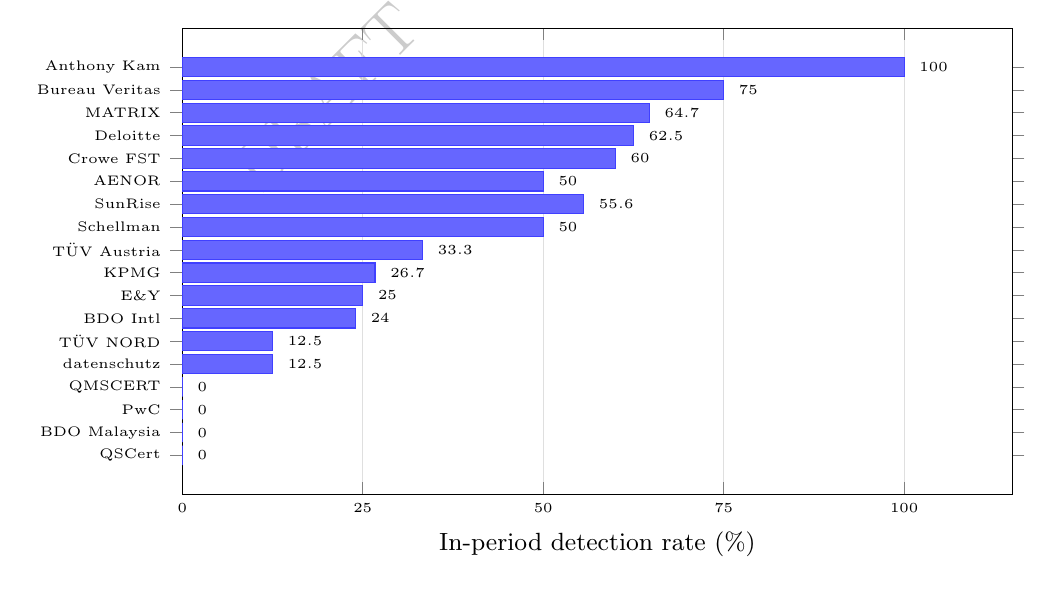
\begin{tikzpicture}
\begin{axis}[
  width=\columnwidth,
  height=7.5cm,
  xbar,
  xlabel={In-period detection rate (\%)},
  symbolic y coords={
    QSCert,BDO Malaysia,PwC,QMSCERT,datenschutz,T\"{U}V NORD,
    BDO Intl,E\&Y,KPMG,T\"{U}V Austria,Schellman,SunRise,
    AENOR,Crowe FST,Deloitte,MATRIX,Bureau Veritas,Anthony Kam},
  ytick=data,
  xmin=0, xmax=115,
  xtick={0,25,50,75,100},
  tick label style={font=\tiny},
  label style={font=\small},
  bar width=7pt,
  xmajorgrids=true,
  grid style={line width=0.3pt, draw=gray!25},
  nodes near coords,
  nodes near coords style={font=\tiny, anchor=west},
  every node near coord/.append style={xshift=2pt},
]
\addplot[fill=blue!60, draw=blue!75] coordinates {
  (100,Anthony Kam)(75,Bureau Veritas)(64.7,MATRIX)(62.5,Deloitte)
  (60,Crowe FST)(55.6,SunRise)(50,AENOR)(50,Schellman)
  (33.3,T\"{U}V Austria)(26.7,KPMG)(25,E\&Y)
  (24,BDO Intl)(12.5,T\"{U}V NORD)(12.5,datenschutz)
  (0,QMSCERT)(0,PwC)(0,BDO Malaysia)(0,QSCert)};
\end{axis}
\end{tikzpicture}
\caption{In-period detection rate by auditor firm (firms with $\geq 3$
in-scope incidents, March 2026). Detection = incident mentioned in the
letter covering the period during which it was filed. Overall rate:
114/390 = 29.2\%. Four firms at 0\%. TayllorCox PCEB has the highest average
letter quality score of any firm with $\geq 3$ clients (84.8/100)
despite zero in-scope incidents, establishing that document quality and
substantive detection are orthogonal.}
\label{fig:detection}
\end{figure}

Three confounders must be stated before interpreting the per-firm spread.
First, the pipeline cannot observe undisclosed matter treatment: a letter
may address an incident's root cause, recommend remediation, or discuss
the underlying condition without naming the specific Bugzilla number.
Such letters score as zero. Second, engagement letter scope may explicitly
exclude certain operational areas; the pipeline cannot determine what was
contractually out of scope for a given engagement. Third, for smaller
firms with few in-scope incidents, small absolute counts (1 in 3 vs.\ 0
in 3) produce large percentage swings that do not reflect systematic
difference in practice.

With those confounders stated, the aggregate finding is robust. The
overall 29.2\% rate is distributed across 390 incident-period pairs and
18 firms. The zero-detection cluster --- four firms, 20 combined
in-scope incidents, zero caught --- is not plausibly explained by scope
exclusions across all seven firms simultaneously. The multi-cycle misses
(36 incidents across two or more consecutive audit cycles) are not
plausibly explained by consistent letter-language differences, since
a pattern-matching failure in one year would not systematically repeat
in the next.

The spread from 100\% to 0\% across firms operating under identical
policy requirements is not random. Three structural properties of the
auditor market predict the direction if not the exact values.

\textit{Engagement model.} The highest-detection firms --- MATRIX,
Anthony Kam, SunRise, AENOR --- are regional specialists with
concentrated WebPKI client bases. A firm whose entire practice is
WebPKI audits develops institutional knowledge of the Bugzilla
incident record, of the CA/B Forum's expectations for incident
disclosure, and of the specific patterns that generate compliance
failures in certificate issuance systems. That knowledge is not a
natural output of a general-purpose assurance practice. For the Big
Four accounting firms --- KPMG, Ernst \& Young, Deloitte --- WebPKI
audits represent a small fraction of a large and varied practice.
The auditors assigned to a WebPKI engagement bring framework expertise
but not necessarily the ecosystem-specific knowledge that correlates
with detecting in-scope incidents.

The multi-cycle miss concentration provides independent corroboration.
BDO International's clients account for 31 of 36 multi-cycle misses
(86.1\%) despite BDO's 30.8\% single-period detection rate being close
to the ecosystem average. A firm that detects incidents at roughly the
ecosystem average in any given period but allows 31 of them to persist
through two or more consecutive audit cycles is not sampling randomly
from the incident population --- it is systematically missing the incidents
that persist. The most parsimonious explanation is the same one that
explains the detection rate spread: absence of a structured per-engagement
Bugzilla review. An auditor who doesn't know to look for open incidents
in year one will not look in year two either.

\textit{Detection methodology.} Detecting in-scope incidents requires
knowing the Bugzilla corpus exists, knowing how to query it, and having
a structured process for checking whether each open bug falls within
the current audit period. This is not specified in WebTrust or ETSI
audit criteria; it is institutional practice. Firms that have built
this check into their engagement process detect incidents; firms that
have not, do not. The 100\% rates for MATRIX and Anthony Kam are most
plausibly explained by a systematic per-engagement Bugzilla review.
The 0\% rates for larger firms are most plausibly explained by its
absence.

\textit{Geographic concentration.} Three of the four zero-detection
firms (QMSCERT, BDO Malaysia, QSCert) serve
primarily ETSI CAs or operate in specific national markets. The
aggregate ETSI detection rate is lower than the WebTrust rate, though
both are below 40\%. Whether this reflects differences in how ETSI
frameworks specify incident disclosure obligations, differences in CA
compliance culture by region, or differences in auditor practice is
not resolvable from the current dataset. It is a finding that warrants
dedicated investigation.

The quality-detection orthogonality finding is particularly instructive.
TayllorCox PCEB's average letter quality score is 84.8/100 --- the highest
among firms with three or more clients --- yet it has zero in-scope
incidents in the retrospective, meaning there were no open Bugzilla bugs
during their clients' audit periods to detect.
LSTI previously illustrated this orthogonality most starkly (zero detection
against high letter quality), but with LSTI's client base now at one parsed letter,
that data point is n=1. The structural pattern holds across the dataset:
letter quality and detection are orthogonal properties of the audit
artifact. High quality measures document structure: unambiguous opinion
statement, current criteria version, correct template use. It does not
measure whether the letter reflects the CA's incident history. An
auditor can produce a formally excellent document that says nothing
about what actually happened.

\subsection{Self-Report Parity Across Frameworks}
\label{sec:selfreport}

WebTrust CAs self-report 56.1\% of their compliance incidents ---
meaning a CA's own staff, linting infrastructure, or internal monitoring
filed the Bugzilla report before any external party identified the
issue. ETSI CAs self-report 61.8\%. The difference is within
measurement noise.

This parity coexists with a meaningful structural difference in letter
quality. ETSI letters average 77.8/100 on the letter quality score
(which measures document structure: opinion clarity, criteria currency,
and template compliance) versus 63.8/100 for WebTrust --- a 14-point
gap. ETSI letters also show scope gap patterns consistent with the overall finding: 12.3\% of all 73 letters (9 of 73) have genuine scope gaps after the S/MIME obligation fix that removed 22 Microsoft-only false positives. The ETSI Audit Attestation Letter (AAL) template
specifies required sections more prescriptively than the WebTrust format,
which likely accounts for the document quality advantage.

The parity in self-report rates, despite ETSI's structural quality
advantage, carries a specific implication. If the framework governed
detection behavior, we would expect different self-report rates.
The parity suggests it does not.

Two structural explanations account for the parity. First, self-report
rates reflect CA behavior, not auditor behavior --- whether the CA's
own monitoring finds the issue before the auditor does is independent
of which framework the auditor uses. Second, the incidents that CAs
self-report are disproportionately governance failures: CPS
non-conformances, disclosure timeline violations, documentation gaps
that CAs identify through internal review cycles. These are not the
kind of technical failures that an auditor's framework methodology
is designed to surface; they are failures the CA discovers by reading
the Baseline Requirements against its own procedures. Under either
WebTrust or ETSI, the CA's internal compliance team is better
positioned than the auditor to find these issues.

The framework quality difference warrants a methodological note on
selection effects. The 18-point quality gap between ETSI and WebTrust
could reflect the frameworks themselves, or it could reflect that
the CAs choosing ETSI are structurally different --- better-resourced,
more compliance-focused, or operating under European regulatory regimes
that impose additional requirements. Thirteen CA owners in the dataset
file both an ETSI letter and a WebTrust letter with CCADB, constituting
a natural within-CA controlled experiment: the same CA, the same audit
period, two different frameworks producing two different letters. Any
difference between the two rows for the same CA is attributable to the
framework and auditor, not to the CA's underlying compliance posture.

The Observatory parses both letters for these 13 dual-framework CAs and
the results are available for three where secondary letter PDFs are
accessible: DigiCert (BDO/WebTrust Q=38.8 vs DQS/ETSI Q=29.4),
PKIoverheid/Logius (KPMG/WebTrust Q=37.5 vs Attestic/ETSI Q=28.1),
and Sectigo (BDO/WebTrust Q=45.0 vs T\"{U}V NORD/ETSI Q=35.6). In all
three cases, the WebTrust letter scores \textit{higher} than the ETSI
letter for the same CA --- the opposite of the population-level
relationship. The most significant within-CA finding is PKIoverheid/Logius:
KPMG issues a qualified opinion on the WebTrust letter while Attestic
issues an unqualified opinion on the ETSI letter covering the same CA.
The same underlying compliance posture, assessed by two auditors under
two frameworks in the same period, produces divergent exception
conclusions. This is the strongest available evidence that the 8.2\%
qualified opinion rate is a property of auditor judgment, not CA
compliance status: the framework does not determine whether the
auditor exercises exception discretion.

On fingerprint coverage, the within-CA comparison confirms that
the population-level ETSI advantage in enumeration (75\% missing
vs.\ 86\% for WebTrust) does not hold at the CA level: both
DigiCert and Sectigo show nearly identical fingerprint miss counts
across their two letters, and PKIoverheid's ETSI letter lists 8
fingerprints while its WebTrust letter lists none --- but both miss 2
trusted roots. The cross-sectional ETSI quality premium appears to
be a composition effect --- ETSI-framework CAs tend to be European,
smaller in scope, and operating under tighter regulatory templates
--- rather than a causal property of the ETSI framework itself.

The ETSI quality advantage therefore does not mean the ETSI framework
produces better incident coupling. On the structural completeness checks
(fingerprint coverage, scope accuracy), ETSI letters perform better
than WebTrust; on substantive detection (whether the letter reflects
the incident record), the framework does not appear to be the primary
variable. The primary variables appear to be CA
internal compliance investment and the specific engagement practice
of the audit firm --- as the per-firm detection spread in
Figure~\ref{fig:detection} confirms. Treating framework choice as
a proxy for audit quality, as some CA compliance guidance does,
is not supported by this data.

\section{Structural Incompleteness}
\label{sec:completeness}

The Web PKI audit system rests on a governance presumption: that the
annual letter a CA submits to CCADB actually covers the roots that
browsers trust, and that the incidents it fails to mention are
genuinely absent from the CA's record. This presumption is what makes
the detection rate finding in Section~\ref{sec:detection} legible as
a compliance failure rather than a scope artifact. If a letter does
not acknowledge incidents that were open during the period, we cannot
verify that the audit function is working.

This is the precondition failure the structural completeness findings
document. The CCADB ALV tool checks two required properties:
whether the letter lists the SHA-256 fingerprints for the root
certificates it covers, and whether it covers all applicable
certificate types. The Observatory computes equivalent checks against
the current CCADB root inventory.

A methodological note: the fingerprint cross-check compares each
letter's fingerprints against the specific roots whose CCADB audit URL
matches that letter's URL --- not all roots for the CA owner. CCADB's
architecture is multi-letter by design: a CA's roots are distributed
across TLS BR, TLS EVG, S/MIME BR, Code Signing, NetSec, and Standard
letter URL columns, and each letter covers only the roots assigned to
its URL. Using all roots for the CA owner as the denominator produces
false positives --- roots legitimately covered by a different letter
type appear as missing from the TLS BR letter. Under the URL-specific
denominator, 82 of 82 parsed TLS BR letters account for all the TLS
roots that CCADB assigns to their URL. The fingerprint enumeration
finding from an earlier version of this analysis (45\%) was an artifact
of the wrong denominator; that finding does not survive methodological
correction.

The scope coverage finding is more durable. Of 73 parsed letters,
9 (12.3\%) fail to cover all certificate types the CA is trusted to
issue, after accounting for separately-filed audit letters. Where a CA
has a distinct Code Signing, S/MIME BR, or TLS EVG letter on file in
CCADB, the TLS letter is not expected to cite those criteria --- correct
practice for large multi-scope CAs. The 11.0\% rate reflects letters
that genuinely omit certificate types the CA is trusted to issue without
a corresponding separate filing. The dominant pattern is S/MIME
capability without a separate S/MIME BR letter: 6 of the 9 CAs with
scope gaps have S/MIME-capable roots in Mozilla but no S/MIME BR audit letter in
CCADB (certSIGN, CFCA, GDCA, GoDaddy, ACCV, and NAVER Cloud Trust Services).
The S/MIME Baseline Requirements became mandatory for Mozilla-included CAs in 2023; these
6 CAs are carrying a trust capability for which no compliant audit
exists. The remaining three scope gap cases involve TLS or Code Signing omissions ---
Chunghwa Telecom (Code Signing capable, no separate Code Signing letter),
Netrust (IMDA criteria does not reference TLS BR), and Trustis (NCP+OVCP only,
no DV coverage). Relying parties cannot verify from these letters that
the audit covered the full scope of what the CA is authorized to do.

A distinct structural finding involves 54 fingerprints across
19 CA letters that match no record in CCADB --- neither root certificate
nor disclosed intermediate. Applying a global lookup across all CCADB
records (not just those filed under the same CA owner) reclassifies 8
as known sub-operator intermediates registered under a parent CA owner;
the remaining 54 are genuinely absent from any CCADB record. These
fingerprints are not in the ecosystem's central transparency database,
yet auditors are attesting to scope over certificates the ecosystem
has never seen. This pattern is consistent with eIDAS-scoped hierarchies
outside the browser root programs, national PKI infrastructure not
disclosed to CCADB, or genuinely undisclosed sub-CA issuance. The
finding is not captured by the ALV tool and does not appear in prior
characterizations of audit incompleteness.

Figure~\ref{fig:alv} shows the per-auditor scope gap rate.
SunRise CPAs/DFK (2 of 5 clients), Auren (1 of 2), and Schellman (1 of 3)
have the highest rates among firms with multiple clients. Firms whose clients are large
commercial CAs that correctly file separate EV, S/MIME BR, and Code
Signing letters show 0\% scope gap rates (BDO International: 0 of 7;
datenschutz cert GmbH: 0 of 2; AENOR: 0 of 4; Deloitte: 0 of 8). Scope gaps concentrate
in two patterns. First, S/MIME capability under Mozilla without a separate S/MIME BR
letter (6 CAs): certSIGN, CFCA, GDCA, GoDaddy, ACCV (Spain), and NAVER Cloud Trust Services,
all included in Mozilla and subject to the S/MIME BR requirement since 2023. Second,
capability-type mismatches --- Chunghwa Telecom
(Code Signing capable, no separate Code Signing letter), Netrust
(IMDA criteria does not reference TLS BR), and Trustis (NCP+OVCP only,
no DV coverage).

\begin{figure}[t]
\centering
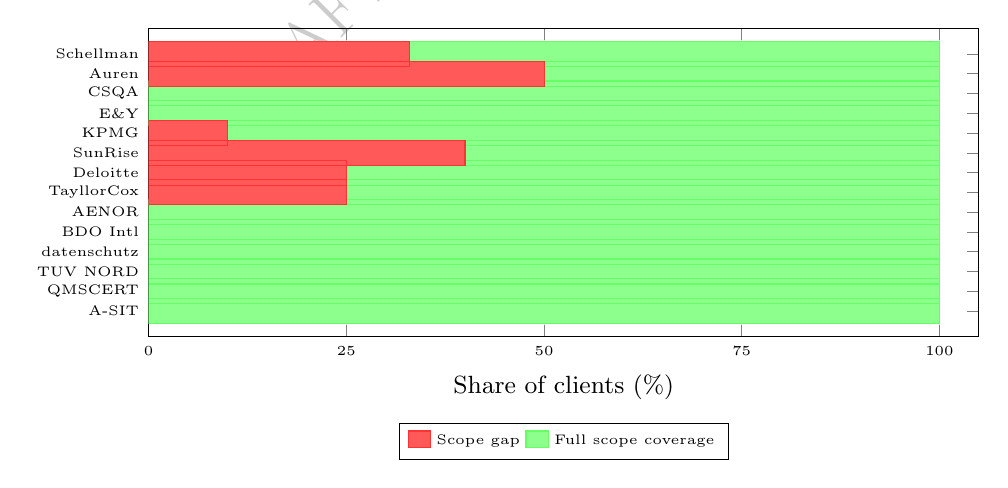
\begin{tikzpicture}
\begin{axis}[
  width=\columnwidth,
  height=5.5cm,
  xbar stacked,
  xlabel={Share of clients (\%)},
  symbolic y coords={
    A-SIT,QMSCERT,TUV NORD,datenschutz,BDO Intl,AENOR,
    TayllorCox,Deloitte,SunRise,KPMG,E\&Y,CSQA,Auren,Schellman},
  ytick=data,
  xmin=0, xmax=105,
  xtick={0,25,50,75,100},
  tick label style={font=\tiny},
  label style={font=\small},
  bar width=9pt,
  xmajorgrids=true,
  grid style={line width=0.3pt, draw=gray!25},
  legend style={font=\tiny, at={(0.5,-0.28)}, anchor=north, legend columns=2},
]
\addplot[fill=red!65, draw=red!80] coordinates {
  (50,Auren)(33,Schellman)(25,TayllorCox)(25,Deloitte)(40,SunRise)
  (10,KPMG)(0,E\&Y)(0,CSQA)(0,AENOR)(0,BDO Intl)(0,datenschutz)(0,TUV NORD)(0,QMSCERT)(0,A-SIT)};
\addlegendentry{Scope gap}
\addplot[fill=green!45, draw=green!60] coordinates {
  (50,Auren)(67,Schellman)(75,TayllorCox)(75,Deloitte)(60,SunRise)
  (90,KPMG)(100,E\&Y)(100,CSQA)(100,AENOR)(100,BDO Intl)(100,datenschutz)(100,TUV NORD)(100,QMSCERT)(100,A-SIT)};
\addlegendentry{Full scope coverage}
\end{axis}
\end{tikzpicture}
\caption{Scope coverage by auditor firm (firms with $\geq 2$ clients,
March 2026). Red = fraction of clients with a scope gap after accounting
for separately-filed per-criteria letters and confirming S/MIME obligation
under an enforcing root program (Mozilla). Gaps reflect S/MIME BR
capability without a corresponding letter (6 CAs), plus TLS/Code Signing
omissions (3 CAs). Of 73 parsed letters, 9 (11.0\%) have scope gaps; 73 (89.0\%) pass
all scope checks.}
\label{fig:alv}
\end{figure}

These findings connect directly to the 2023 theoretical
prediction~\cite{hurst2023} that auditors are ``essentially tasked
with assessing if the checklist represented in the audit regime can
be reasonably deemed as met.'' The checklist can be satisfied ---
ALV passes, the opinion is issued, the letter is filed --- while
6 CAs carry an S/MIME trust capability for which the now-mandatory
audit does not exist, and 19 CA letters attest to scope over fingerprints
the ecosystem has never registered.

The third required property --- incident cross-references --- is not
checked by ALV at all. CCADB Policy \S5 requires that letters cover
incidents open during the period, but no automated tool at submission
time verifies that the letter mentions them. The Observatory provides
that check; Section~\ref{sec:detection} measures the result. The
structural incompleteness findings and the detection rate findings
are therefore not parallel observations about the same system ---
they are a hierarchy. Scope incompleteness means the letter cannot
establish what it purports to cover. Incident omission
means the letter fails to report what happened within the scope it
does claim. A relying party reading an incomplete letter that also
omits in-period incidents has not received a weaker assurance. They
have received something that does not function as assurance at all.

\section{The Denominator Problem}
\label{sec:denominator}

The 29.2\% detection rate uses a denominator that is smaller than the
policy-mandated scope. CCADB Policy \S5.1~\cite{ccadb-policy} states
that audit letters must cover all incidents that ``at any time during
the audit period, occurred, were open in Bugzilla, or were reported
to a Root Store Operator.'' This includes incidents filed before the
audit period started that remained open when the period began.

The Observatory's denominator counts only incidents filed \textit{during}
the period --- it does not include pre-existing open incidents because
Bugzilla's public API does not expose resolution dates. The full
policy-mandated denominator would add every incident that was
unresolved at the start of each audit period, regardless of when it
was filed.

An illustrative case: a CA with a compliance failure first identified
in 2020 and not fully remediated until 2023 should appear in the
2020--2021 letter, the 2021--2022 letter, and the 2022--2023 letter.
Our measurement captures only the first period (the one containing
the filing date). The subsequent periods --- where the incident was
open but pre-dates the period --- are excluded from both numerator
and denominator. If the later periods' letters do not mention the
incident, the miss is invisible to our measurement.

The DER-to-PEM encoding failures documented in Bugzilla across
multiple CAs (e.g., Netlock Bug 2004699, December 2025) illustrate
the pattern: a class of technical failure that persists across years
should appear in consecutive audit letters. Our instrument detects
the failure only in the period containing the initial filing.

The consequence is clear: 29.2\% is an upper bound on the true
detection rate. The actual rate of compliance with CCADB Policy \S5's
disclosure requirement is lower, by an amount we cannot quantify
without resolution-date data. Future work extending the pipeline to
capture bug resolution dates through the Bugzilla REST API's
\texttt{last\_change\_time} field would allow computation of the full
policy-mandated denominator.

\section{Clean Opinions During Documented Decay}
\label{sec:opinions}

Of 73 parsed audit letters, 6 (8.2\%) carry qualified opinions ---
auditors who could not fully certify compliance issued exception
notices. Swiss BIT (KPMG), PKIoverheid/Logius (KPMG), Entrust
(Deloitte), e-commerce monitoring GmbH (A-SIT), the Finnish
Population Register Centre (QMSCERT), and Microsoft Corporation
(KPMG) are the six.

The composition of the qualified-opinion group is structurally
informative. Five of the six are government-operated or public-sector CAs ---
Swiss federal, Netherlands, Finland, e-commerce monitoring (Austria),
and Microsoft PKI Services (a CA operated by a corporation rather
than a government, but with the accountability structure of a major
technology vendor). The sixth is Entrust, the only commercially-operated CA
in the group and the only one that subsequently underwent distrust
proceedings (2024). The pattern is not that qualified opinions are
uniformly distributed across the CA population; they are concentrated
in CAs with structural accountability relationships to national
regulators that create external pressure for exception acknowledgment,
and in the one commercial CA whose compliance pattern eventually
triggered enforcement action. The 67 CAs with unqualified
opinions include DigiCert (171 incidents), Sectigo (109), and
IdenTrust (68).

The remaining 67 carry unqualified opinions. This 91.8\% clean
opinion rate coexists with a 29.2\% incident detection rate, a 34.8\%
audit staleness rate (stale or very stale: 31 of 89 CA owners), and
38 of 39 CAs with retrospective data showing a high transparency gap
(the letter cross-references fewer than 20\% of the CA's all-time incident history).

Letter quality scores (0--100, scored against the standard in effect
at audit time) show a mean of 69.4/100 across 73 parsed letters, with
a distribution: 20 letters grade A ($\geq$90), 1 grade B,
10 grade C, 24 grade D, and 18 grade F. The distribution shows a cluster
of high-quality letters concentrated in smaller regional specialists
and a middle band of C-grade letters from the larger global firms, with
relatively few at the extremes below C.
The mean of 69.3 (C+) masks this spread. As Section~\ref{sec:detection-firms} establishes,
neither high nor low quality scores predict detection rates --- the
A-grade firms and the F-grade firms have overlapping detection
rate distributions.

Table~\ref{tab:highgap} shows the five CAs with the largest all-time
incident histories and their current transparency gap scores. DigiCert
(171 incidents, gap 98.2\%), Sectigo (109 incidents, gap 98.2\%),
IdenTrust (68 incidents, gap 95.6\%), SwissSign (63 incidents, gap
93.7\%), and GlobalSign (55 incidents, gap 90.9\%) each have
all-time incident histories that the current letter cross-references
at under 10\%. All five carry unqualified opinions.

\begin{table}[t]
\centering
\footnotesize
\setlength{\tabcolsep}{3pt}
\caption{High-incident CAs and transparency gap (March 2026). Gap =
fraction of all-time Bugzilla incidents not mentioned in any audit letter.
All five carry unqualified (clean) audit opinions.}
\label{tab:highgap}
\begin{tabularx}{\columnwidth}{@{}Xrrr@{}}
\toprule
CA & Inc. & Gap & Auditor \\
\midrule
DigiCert             & 171 & 84.2\% & BDO Intl \\
Sectigo              & 109 & 90.8\% & BDO Intl \\
IdenTrust            &  68 & 95.6\% & BDO Intl \\
SwissSign            &  63 & 88.9\% & T\"{U}V Austria \\
GlobalSign           &  55 & 92.7\% & KPMG \\
\bottomrule
\end{tabularx}
\end{table}

The transparency gap is not a per-letter detection metric ---
it compares all-time history against the current letter only, so
a long-tenured CA will mechanically show a higher gap than a new one.
But the combination is telling: the largest and most active CAs in
the ecosystem, with the longest compliance histories and the most
incidents on record, produce current letters that auditors certify
as clean while cross-referencing under 10\% of that history.

A related structural inversion is visible across the market. The
five CA owners with the largest issuance share --- ISRG (39.8\%),
Google Trust Services (16.2\%), DigiCert (14.0\%), GoDaddy (13.0\%),
and Sectigo (10.8\%), collectively covering 93.8\% of all unexpired
certificates --- produce letter quality scores of 52.5, 65.6, 38.8, 38.8, and 45.0 respectively,
all below the 69.3 mean. The fingerprint enumeration check passes for all of
these CAs after correctly restricting the denominator to TLS-capable roots
assigned to each letter's specific URL. The quality inversion remains:
firms auditing higher-volume, more automated issuance infrastructure
systematically produce weaker letters. This is not an artifact of CA type or size ---
it is a structural property of the relationship between dominant-CA
issuance model and audit engagement depth. A CA producing 40\% of
the world's TLS certificates under a fully automated renewal pipeline
does not present the same audit surface as a CA producing 0.1\% under
a manually-managed enterprise model.

The 2025 theoretical work~\cite{hurst2025} states: ``almost every distrusted
CA had passing audit reports. Nearly all of them showed years of
compliance issues before trust was revoked.'' The Observatory now
measures this directly. Among the 16 distrusted CAs in the dataset,
10 have Bugzilla compliance histories; of those, 2 have CCADB audit
timelines that overlap the compliance failure period. The small overlap
count ($n=2$) is a data constraint, not a finding: most distrusts
predate systematic CCADB audit record collection, and several distrusted
CAs' CCADB records post-date their failure periods. For those two,
the in-period audit detection rate is 7.5\%: Deloitte issued a
qualified opinion on Entrust while 27 in-scope incidents were open
and caught 3 (11.1\%); LSTI, whose zero detection rate is documented
in Section~\ref{sec:detection-firms}, audited Certinomis across a
period covering 13 in-scope incidents and caught none. The remaining
8 distrusted CAs either have no CCADB audit records (removed before
current data collection) or have records that post-date the compliance
failures --- the letters that should have caught the issues are not
in CCADB. The 7.5\% figure is therefore a ceiling on what is
measurable from two cases, not a floor on how much was missed across
the full distrust record. The high-gap,
clean-opinion combination is the audit-letter signature of the
``gradually'' phase --- compliance issues accumulating while formal
attestations say otherwise.

\section{Auditor Selection and the 2025 Spike}
\label{sec:switches}

Between 2015 and 2024, the number of CA auditor switches per year
averaged 2--4. In 2025, 21 switches occurred --- a five-fold increase
against the historical baseline. Four additional switches occurred in
early 2026.

The most parsimonious explanation for the spike is the ETSI EN 319 411
v3.5 recertification requirement that took effect in March 2026. ETSI
CAs whose incumbent auditors had not yet obtained v3.5 accreditation
were required to switch to accredited firms. The switches were
regulatory mandate, not discretionary quality signals.

This matters for the interpretation of auditor quality comparisons.
If CAs select auditors primarily to satisfy accreditation requirements
rather than to maximize detection quality, the market mechanism that
would reward high-detection firms and penalize low-detection ones
does not operate. The 2025 spike provides a natural experiment:
switches driven by mandatory recertification cannot be interpreted
as votes of confidence or no-confidence in the incumbent firm's
detection performance.

Figure~\ref{fig:switches} shows the annual switch count. The
HHI for the audit services market is 557.9 --- unconcentrated by
standard DoJ/FTC thresholds ($<$1,500), with KPMG (10 clients),
Deloitte (8 clients), and BDO International (7 clients) as the three
largest firms. Low aggregate concentration does not mean individual
firm exits are costless: KPMG's 10 clients represent 11.4\% of the
named market, and its exit would require those CAs to switch to a
much smaller pool of accredited alternatives. The 2025 switch spike
temporarily redistributed approximately one-quarter of the ETSI
client base across that constrained pool.

\begin{figure}[t]
\centering
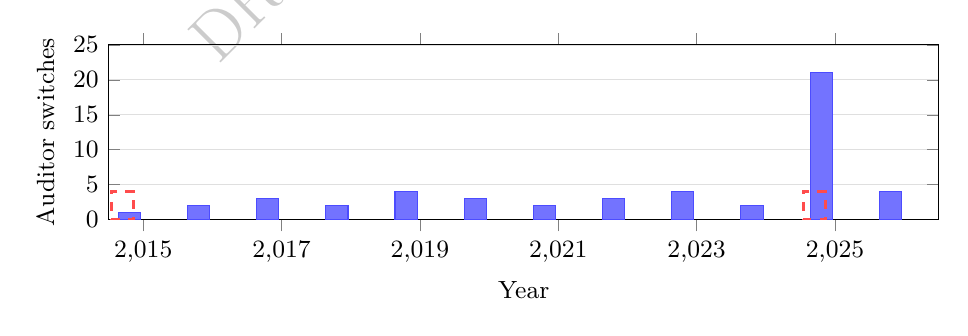
\begin{tikzpicture}
\begin{axis}[
  width=\columnwidth,
  height=3.8cm,
  ybar,
  xlabel={Year},
  ylabel={Auditor switches},
  xmin=2014.5, xmax=2026.5,
  ymin=0, ymax=25,
  xtick={2015,2017,2019,2021,2023,2025},
  ytick={0,5,10,15,20,25},
  tick label style={font=\small},
  label style={font=\small},
  bar width=8pt,
  ymajorgrids=true,
  grid style={line width=0.3pt, draw=gray!25},
]
\addplot[fill=blue!55, draw=blue!70] coordinates {
  (2015,1)(2016,2)(2017,3)(2018,2)(2019,4)(2020,3)
  (2021,2)(2022,3)(2023,4)(2024,2)(2025,21)(2026,4)};
\addplot[dashed, no marks, very thick, color=red!70] coordinates {
  (2014.5,4)(2024.5,4)};
\end{axis}
\end{tikzpicture}
\caption{Annual auditor switch count (2015--2026 partial). Dashed line
shows the 2015--2024 mean ($\approx$2--4/year). The 2025 spike (21
switches, five-fold increase) coincides with the ETSI EN 319 411 v3.5
recertification requirement taking effect in March 2026, which required
ETSI CAs to switch to v3.5-accredited firms. Four further switches
occurred in early 2026.}
\label{fig:switches}
\end{figure}

\subsection{The Natural Experiment}
\label{sec:switches-experiment}

The 2025 spike provides a rare opportunity to test whether auditor
switches improve audit-incident coupling. Of the 21 switches, 9 were
ETSI-framework CAs and 12 were WebTrust. The ETSI switches are the
natural experiment: driven by mandatory v3.5 recertification, they
are exogenous to any quality signal from incumbent performance.

Among the 15 switches where both the incoming and outgoing firm had
parsed letters allowing letter-quality comparison: 6 switched to a
lower-scoring firm, 5 to a higher-scoring firm, and 4 were neutral.
The accreditation-driven ETSI switches show no systematic improvement
in letter quality: certSIGN moved from LSTI (historically high letter quality,
now n=1 parsed letter) to
Crowe FST Audit Ltd\ (delta $-34.8$ points versus prior LSTI average); Izenpe moved from LSTI
to AENOR (delta $-12.9$); Telia moved from KPMG to datenschutz cert
GmbH (delta $+14.2$). Finland moved from datenschutz cert GmbH to
QMSCERT ($+1.7$).

Two findings follow. First, the mandatory recertification did not
systematically select for higher-quality incoming auditors ---
switches were constrained by v3.5 accreditation availability, not
quality optimization. Second, and more important, per-letter quality
scores are not the primary quality signal that matters: as
Section~\ref{sec:detection-firms} establishes, document quality and
substantive incident detection are orthogonal. CAs that switched away from LSTI
for accreditation reasons may have moved to firms with lower document
quality scores but equal or better incident coupling --- that comparison
requires per-letter incident data that the current pipeline does not
yet capture at the switch level.

The natural experiment has additional potential that the current
data does not yet fully exploit. If the 21 switched CAs' post-switch
incident coupling can be measured in 2026 audit letters (now being
filed), the switch event provides a clean pre/post comparison for
the same CA under different auditors. This would be the first
empirical test of whether auditor choice causally affects detection
rates in the WebPKI context. The Observatory's daily pipeline is
positioned to run this comparison automatically as 2026 letters
are submitted to CCADB, producing a prospective quasi-experimental
dataset within 12 months.

The broader implication is structural: if the primary driver of
auditor selection is regulatory accreditation compliance rather than
detection quality, the market mechanism that would reward
high-detection firms cannot function. CAs have limited ability to
select on detection quality because (a) detection rates are not
published, (b) accreditation availability constrains the choice set,
and (c) the audit engagement is priced and scoped before detection
outcomes are observable.
\label{sec:discuss}

\subsection{Why the Coupling Failure Is Self-Reinforcing}

Clinical diagnostic testing distinguishes sensitivity (true positive
rate) from specificity (true negative rate) for good reason: a test
optimized purely for specificity can issue clean results on diseased
patients without lying, if its detection criteria are narrow enough.
The audit system the data describes has optimized for specificity in
a specific sense: it reliably produces clean opinions for CAs that
are not in active crisis, while detecting 29.2\% of the incidents that
were open and documented in a public database during the audit period.

This is not auditor failure in the ordinary sense. It is the predictable
output of a system with known incentive properties. The 2023
work~\cite{hurst2023} names them: the auditor is retained by the auditee,
the scope is defined by mutual agreement, the sample is selected under
conditions the auditee helps set, and the product is a document that
satisfies a procurement requirement rather than a risk assessment. Under
those conditions, the rational audit strategy is to produce a
well-structured document that satisfies the engagement criteria as
scoped, without over-reaching into areas outside the contracted scope. The 29.2\% detection rate and the 11.0\% scope gap rate are not evidence that auditors
are cutting corners; they are
evidence that the system is operating exactly as its incentive structure
predicts.

The pharmaceutical clinical trial literature provides an instructive
analogy. Trials sponsored by the manufacturer of the drug being tested
show systematically more favorable outcomes than independent trials ---
not because researchers fabricate data, but because sponsor-controlled
design choices (comparator selection, endpoint definition, follow-up
duration) accumulate to produce a systematic bias. No individual
decision is fraudulent; the aggregate outcome is structurally
predictable. The audit system exhibits the same property: no individual
auditor is lying, and the aggregate outcome --- 29.2\% detection across
73 letters --- is structurally predictable from the design.

The analogy holds at the regulatory response level too. The
pharmaceutical industry's answer to sponsor bias was not to impugn
individual researchers but to mandate pre-registration of trial
protocols, require publication of negative results, and establish
independent data safety monitoring boards with authority to review
unblinded data against pre-specified stopping rules. Each of these
interventions targets a specific structural property: pre-registration
prevents endpoint switching; negative result publication removes
publication bias; independent monitoring boards remove the sponsor's
ability to select what the regulator sees. The WebPKI's equivalent
interventions are visible in the recommendations in
Section~\ref{sec:remedies}: mandatory Bugzilla cross-referencing
removes the auditor's discretion over which incidents to acknowledge;
published detection rates create the external accountability that
internal engagement incentives suppress; the Observatory's continuous
measurement plays the role of the independent monitoring board,
generating data the parties to the audit engagement do not control.

The analogy also identifies where the parallel breaks down, and the
break is instructive. Pharmaceutical trials have an independent
regulator --- the FDA, EMA, or equivalent --- with statutory authority
to require protocol changes and withhold product approval. The WebPKI
has root programs with significant practical authority but no statutory
mandate, operating under voluntary governance with no minimum
participation requirements. The interventions that work in the
pharmaceutical context require an authority willing and able to impose
them. The browser root programs demonstrated that authority exists in
the Entrust and Symantec distrusts; whether they will use it to mandate
audit quality requirements is the open question the data this paper
presents makes harder to defer.

But the mechanism already exists. CCADB Policy is maintained and updated
by the root programs themselves --- it requires no new legislation, no new
institution, and no new authority. Adding mandatory Bugzilla citation for
in-scope incidents to CCADB Policy \S5 would convert the detection requirement
from an aspirational disclosure expectation into a mechanically verifiable
submission check. The ALV tool already validates fingerprint enumeration
and scope coverage at submission time. The Observatory already computes
the incident cross-reference check. Making that check run at submission
rather than post-hoc requires a policy amendment, not a new law.
The pharmaceutical analogy breaks down on statutory authority; it does
not break down on mechanism. The root programs have the mechanism.
The data this paper presents establishes that the current policy
requirement is not being met, at a rate that is now measurable and public.
Whether to close that gap is a governance choice, not a technical
constraint.

A third structural factor compounds the incentive problem: the
regulatory surface that auditors are certifying against has grown
122-fold since the audit framework was introduced, while the
engagement model has not changed. In 2000, CA compliance could be
characterized against approximately 55 total requirements. By 2026,
the WebPKI Observatory measures 6,706 active obligations across
CA/B Forum standards, root program requirements, audit framework
criteria, and regulatory instruments~\cite{snapshot} --- with
mandatory obligations alone reaching 5,095. The TLS Baseline
Requirements, which define the core of what WebTrust and ETSI
auditors certify against, grew from 278 requirements at v1.0 in
2012 to 1,317 today (4.7$\times$), with the largest single-year
additions occurring in 2021 (+899 mandatory obligations), 2023
(+459), and 2024 (+1,580). The annual letter format, the
once-per-year engagement frequency, the auditor-day budget, and the
scope definition process have not scaled proportionally.

This is not a peripheral observation. It is the structural explanation
for why the per-firm detection spread documented in
Section~\ref{sec:detection-firms} follows a pattern that mirrors
WebPKI-specific institutional knowledge rather than auditor size or
resources. A skilled generalist auditor working from the ETSI or
WebTrust criteria checklist in 2000 could hold the entire obligation
surface in working memory. The same audit methodology in 2026
operates against a surface 122 times larger without a corresponding
expansion in the depth of per-obligation verification. The compliance
obligation surface auditors certify against grew from 55 discrete
requirements in 2000 to 6,706 by 2026 --- a 122$\times$ expansion,
with 76\% mandatory --- while the engagement model (once-per-year
review, fixed-day budget, same letter format) did not change. The
incidents that go undetected are not random: they are the incidents that require
ecosystem-specific knowledge of the Bugzilla corpus, the CA/B Forum
policy history, and the specific failure patterns that the criteria
checklists were written to prevent --- knowledge that scales with
WebPKI practice concentration, not with audit firm size.

The 2025 theoretical work~\cite{hurst2025} makes the organizational dynamics explicit.
The compliance team that knows the processes are brittle lacks the
authority to halt issuance. The engineering team that knows the controls
are failing is rewarded for velocity, not compliance. Leadership knows
there are findings but faces market share pressure. The auditor, aware
that producing too many findings creates friction, operates reasonably
within the engagement scope. Everyone is locally rational; the system
is globally fragile. The 36 multi-cycle misses --- incidents that
traversed two or more consecutive annual audit cycles unacknowledged
in any letter --- are the audit record of that dynamic.

\subsection{The Compound Failure}

Longitudinal measurement of root program Bugzilla engagement~\cite{sister}
shows that Chrome's Bugzilla oversight coverage peaked at 67.8\% in 2019 and fell
to 18.4\% in 2025; Mozilla's peaked at 86.2\% in 2017 and fell to 9.9\%
in 2025, with neither program having recovered to prior levels. This paper
documents that the formal audit system detects 29.2\% of in-scope incidents.
These are not independent findings.

The Web PKI's compliance architecture has two mechanisms for catching
failures: external oversight by root programs and formal annual audits
by accredited third parties. The governance measurement shows the first is
degraded. This paper shows the second detects less than a third of
what it is responsible for covering. Together, they establish that
the ecosystem's detection capacity is now primarily dependent on a
third mechanism that was not designed to carry this load: CA
self-monitoring. Longitudinal discovery channel data shows CA self-filing
reached 46.1\% of incidents in 2025 and 43.2\% in 2026~Q1~\cite{sister}.

The root program oversight degradation has a specific structural property
that amplifies this paper's findings. Chrome's Bugzilla oversight is 87\%
attributable to a single individual (97\% to the top three contributors across 6
total); Mozilla's is 47\% from one contributor (90\% from three,
across 9 total). When those dominant
contributors reduced engagement in 2020 (Mozilla) and 2022 (Chrome),
oversight coverage fell to its lowest measured levels. This concentration
means the root program oversight that would otherwise validate or
challenge clean audit opinions on high-incident CAs was functionally
absent at the same time the 29.2\% detection rate was being
generated. The two failures are not independent: they are simultaneously
degraded components of a system that was designed assuming both
would function.

The ecosystem is adapting to the degradation of both formal mechanisms
by internalizing detection. This is a genuine positive signal where
it is happening. The asymmetry is significant: self-monitoring is
concentrated in the well-resourced CAs with dedicated compliance teams
and internal tooling. The tail CAs
with the highest per-certificate failure rates
are precisely the
ones least likely to have built the internal monitoring capacity that
can substitute for external oversight and formal audit detection.

\subsection{Compliance at the Speed of Code}
\label{sec:ai}

The formal denominator gap established in
Section~\ref{sec:denominator-method} --- $D_\text{measured} \subset
D_\text{policy}$ --- reflects a structural property of the current
measurement instrument: it cannot observe pre-existing open incidents
or incidents reported outside Bugzilla. AI-generated compliance
artifacts introduce three additional mechanisms that expand this gap
in ways the audit architecture has not been designed to handle.

AI agents are already generating compliance artifacts. Incident reports
are drafted by language models and submitted by humans who may or may
not review them substantively. CPS updates are produced by agents
trained on template libraries. Root cause analyses are generated from
structured inputs. The trajectory is clear: within the next several
years, the artifacts that auditors review will be produced at machine
speed --- not annually but continuously, not by humans with institutional
memory of the incident but by agents optimized to produce plausible
compliance language.

This creates a compound problem. An audit system that detects 29.2\% of
known failures when artifacts are written by humans and reviewed annually
will not improve when those artifacts are generated by systems that can
produce any desired output instantly and at scale.

Three specific properties of AI-speed compliance generation each expand
$D_\text{policy} \setminus D_\text{measured}$ --- the incidents that
policy requires disclosure of but the measurement instrument cannot see:

\textit{Volume and pattern masking.} The distrust cases in the companion
paper~\cite{sister} share a common structure: compliance decay accumulated
gradually over years before triggering sudden enforcement action. The
``gradually'' phase was detectable because human-authored artifacts carry
behavioral signatures of institutional stress --- recurring root cause
language, escalating scope qualifications, inconsistencies between
successive CPS versions, remediation commitments that do not address
the identified failure mode. These patterns are what root program
reviewers, researchers, and eventually auditors used to distinguish a
CA whose operations were degrading from one having isolated incidents.
AI-generated compliance artifacts are syntactically uniform regardless
of underlying operational state. A language model prompted to produce
a root cause analysis for a CA in active compliance decay will generate
the same well-structured, BR-citing, remediation-proposing document as
one generated for a CA operating normally. The behavioral drift signal
that made the ``gradually'' phase visible gets homogenized away.
$D_\text{measured}$ shrinks not only because auditor bandwidth is
fixed while nominal artifact volume grows, but because the signal
that previously pushed incidents into $D_\text{measured}$ through
pattern recognition --- the signal that compliance was accumulating,
not resolving --- disappears into syntactic uniformity. What arrives
suddenly will no longer have been gradual in any detectable sense.

\textit{Plausibility.} $D_\text{measured}$ currently benefits from
an implicit consistency check: human-authored compliance artifacts
are often detectable as inconsistent when something is being concealed.
The root cause analysis contradicts the incident timeline; the corrective
action does not address the identified failure mode; the CPS description
does not match the operational procedure. AI-generated artifacts are
syntactically consistent by construction. A well-prompted language model
will produce a root cause analysis that is internally coherent, cites
the correct BR sections, and proposes plausible remediation regardless
of whether any of it reflects what actually happened. The implicit
signal that pushes incidents into $D_\text{measured}$ through
inconsistency detection disappears.

\textit{Attribution.} $D_\text{measured}$ relies on the traceability
of the artifact to a human author with professional accountability.
When artifacts are generated by agents, the record exists but its
provenance is different: it reflects what the agent was prompted to
say, not what the responsible engineers understood about the incident.
Attribution of accountability becomes harder, which makes the
escalation pathway from detected incident to enforcement action
longer and more uncertain.

The implication is not that AI-generated compliance artifacts are
inherently dishonest. It is that an audit system designed to review
human-generated artifacts of known volume and limited plausibility has
not been designed for the artifact environment it is about to encounter.
The 29.2\% detection rate at human scale is the baseline $\hat{\rho}$
from which AI-speed compliance begins. Without architectural change ---
continuous automated verification against independent signals, mandatory
cross-referencing against the public Bugzilla record, detection rate
measurement as a published audit quality metric --- $\hat{\rho}$ will
decline as artifact volume increases and the auditor's review
depth per artifact decreases.

\subsection{What the Audit System Would Need to Change}
\label{sec:remedies}

Three changes would materially improve detection at both human and
machine timescales.

\textit{Mandatory Bugzilla cross-referencing.} CCADB Policy \S5 already
requires disclosure of all in-scope incidents. Making compliance
with this requirement mechanically verifiable --- by requiring explicit
Bugzilla citation for every in-scope incident, not just the ones
auditors identify independently --- would convert the detection
requirement from a qualitative judgment call into a structured data
check. The Observatory already performs this check at the per-incident
level. The ALV tool already runs equivalent checks on fingerprints and
scope at submission time. Extending ALV to verify incident
cross-references requires a CCADB Policy amendment and an ALV
implementation update --- both within the root programs' existing
authority and tooling infrastructure, neither requiring statutory action
or new governance bodies.

\textit{Detection rate as a published audit quality metric.} No root
program currently publishes detection rates by auditor firm. The data
exists --- Bugzilla is public, CCADB audit records are public, the
matching is computable. Publishing per-auditor detection rates
annually would create a reputational incentive that does not currently
exist. CAs would have a basis for selecting auditors on detection
quality; root programs would have a basis for conditioning CA
acceptance on minimum detection thresholds.

\textit{Resolution-date corpus.} Extending the Bugzilla data pipeline
to capture bug resolution dates would allow computation of the full
CCADB Policy \S5 denominator --- all incidents that were open at any
point during the audit period, regardless of filing date. This is
the denominator the policy requires; it is the denominator the audit
system should be measured against. The Observatory can implement this
with one API field addition.

\section{Conclusion}
\label{sec:conclusion}

The audit-incident coupling gap documented in this paper is not a
performance shortfall that better-motivated auditors would close.
It is a structural property of the formal assurance system ---
measurable, reproducible, and predicted from first principles by the
incentive analysis in prior work~\cite{hurst2023, hurst2025} before
any measurement existed. The data confirms the predictions: 29.2\%
in-period detection against a denominator that is itself an upper
bound, 36 incidents surviving repeated formal review, 9 of 73 parsed letters
with scope gaps (certificate types trusted but unaudited), 6 qualified opinions (8.2\%).
A system producing these outputs is not underperforming; it is
performing as designed.

What the measurement adds to the prior theoretical argument is
verifiability. The 2023 work~\cite{hurst2023} identified five
structural properties that predict systematic underdetection. The 2025
work~\cite{hurst2025} observed that almost every distrusted CA had passing
audit reports. This paper establishes the rate at which the underdetection
occurs, the distribution of that rate across the auditor market, the
formal relationship between what the measurement instrument can
compute ($D_\text{measured}$) and what the policy requires
($D_\text{policy}$), and --- for the first time --- a direct measurement
of audit detection rates during the compliance failure periods that
preceded CA distrust. That rate is 7.5\%: 3 of 40 in-scope incidents
caught across the two distrusted CAs where audit periods and bug
histories overlap ($n=2$, constrained by CCADB coverage predating
most distrust events). The gap $D_\text{policy} \setminus D_\text{measured}$
is not a data artifact; it is the space in which accumulated compliance
failures persist unacknowledged while formal attestations say otherwise
--- including the failures that ultimately end in removal from trust.

The compound failure documented across the two Observatory papers~\cite{sister}
---~external oversight declining, formal audit detection at 29.2\%,
CA self-monitoring as the residual load-bearing mechanism --- means the
ecosystem's compliance detection infrastructure depends structurally
on the goodwill and investment of the CAs themselves. That is a
reasonable outcome in a well-resourced ecosystem with strong internal
compliance culture. It is a fragile outcome in an ecosystem that
includes 74 tail CAs with per-certificate failure rates more than a
thousand times the head, most of which have not built the internal
monitoring capacity that makes self-detection possible.

The AI-speed compliance transition does not change these structural
properties. It stresses them. When the artifacts that auditors review
are generated at machine speed by systems optimized for plausible
compliance language, $\hat{\rho} = 29.2\%$ is the floor from which
the system enters that transition --- and each of the three AI-specific
mechanisms identified in Section~\ref{sec:ai} expands
$D_\text{policy} \setminus D_\text{measured}$ further. Making
$\hat{\rho}$ a published, measured, policy-relevant number is the
precondition for the architectural changes that transition will require.

The Merkle Tree Certificates transition reinforces the stakes. During
the 15--20 year dual-issuance period, every CA must provision both
X.509 and MTC pipelines, each subject to separate audit scope and
incident obligations. The audit letters that will certify MTC issuance
log operations will be produced by the same firms, under the same
incentive structures, that produced these results for X.509. CCADB
Policy's disclosure requirements will apply to MTC incidents with the
same denominator problem: incidents open during the audit period but
filed before it began will not appear in $D_\text{measured}$. The
29.2\% detection rate, the 12.3\% scope gap rate, and the
four zero-detection firms are not legacy properties that the MTC
transition will leave behind. They are the baseline conditions under
which MTC audit oversight will begin.

\bibliographystyle{plain}
\begin{thebibliography}{10}

\bibitem{sister}
Research.
\newblock Unmonitored by Design: A Longitudinal Measurement Study of
  Governance Failure in the Web PKI.
\newblock Systematic Reasoning, Inc., Working Draft, 2026.

\bibitem{snapshot}
WebPKI Observatory LLM Snapshot.
\newblock \url{https://webpki.systematicreasoning.com/llm_snapshot.json},
  March 2026.

\bibitem{github}
WebPKI Observatory Source Repository.
\newblock \url{https://github.com/systematicreasoning/webpki-observatory}.

\bibitem{hurst2023}
R.~Hurst.
\newblock The Limitations of Audits.
\newblock \textit{Unmitigated Risk}, February 2023.
\newblock \url{https://unmitigatedrisk.com/?p=717}.

\bibitem{hurst2025}
R.~Hurst.
\newblock Gradually, Then Suddenly: Compliance as a Vital Sign of
  Organizational Decay.
\newblock \textit{Unmitigated Risk}, October 2025.
\newblock \url{https://unmitigatedrisk.com/?p=1103}.

\bibitem{ccadb-policy}
Mozilla.
\newblock Common CA Database Policy.
\newblock \url{https://www.ccadb.org/policy}, 2026.

\bibitem{ccadb-alv}
Mozilla / Microsoft.
\newblock CCADB Audit Letter Validation Documentation.
\newblock \url{https://www.ccadb.org/cas/alv}, 2026.

\bibitem{webtrust}
CPA Canada / AICPA.
\newblock WebTrust for Certification Authorities --- SSL Baseline with Network
  Security.
\newblock Version 2.7.1, 2024.

\bibitem{etsi-en}
ETSI.
\newblock EN 319 411-1: Electronic Signatures and Infrastructures --- Policy
  and Security Requirements for Trust Service Providers Issuing Certificates.
\newblock Version 1.3.1, 2021.

\bibitem{amann2017}
B.~Amann, J.~Amann, A.~Vallentin, and R.~Sommer.
\newblock Mission Accomplished? HTTPS Security after DigiNotar.
\newblock In \textit{Proceedings of the ACM Internet Measurement Conference
  (IMC)}, 2017.

\bibitem{liu2015}
B.~Liu, S.~Antonakakis, M.~Antonakakis, X.~Xu, and A.~Snoeren.
\newblock An End-to-End Measurement of Certificate Revocation in the Web's PKI.
\newblock In \textit{Proceedings of the ACM Internet Measurement Conference
  (IMC)}, 2015.

\bibitem{durumeric2013}
Z.~Durumeric, J.~Kasten, M.~Bailey, and J.~A. Halderman.
\newblock Analysis of the HTTPS Certificate Ecosystem.
\newblock In \textit{Proceedings of the ACM Internet Measurement Conference
  (IMC)}, 2013.

\bibitem{sun2024}
Y.~Sun, A.~Cowie, R.~Holz, and P.~Zimmermann.
\newblock Revisiting Certificate Transparency: What Has Changed Since 2015?
\newblock In \textit{Proceedings of the Network and Distributed System
  Security Symposium (NDSS)}, 2024.

\end{thebibliography}

\end{document}
